\documentclass[11pt,letterpaper]{article}
\usepackage{fullpage}

\usepackage[english]{babel}
\usepackage[utf8]{inputenc}
\usepackage{amsmath}
\usepackage{graphicx}
\usepackage[hidelinks]{hyperref}
\usepackage{float}
\usepackage{amsfonts}
\usepackage{algorithm,algpseudocode}
\usepackage{pdfpages}
             
\graphicspath{{../results}}

\begin{document} 

\title{Competing Bandits}
\maketitle

\section*{Overview of Results}

First, summarizing the simulation results that we have seen:

\textbf{Priors}:
\begin{enumerate}
\item Needle In a Haystack (x, K) = (K-1) arms with a mean of x and 1 arm with mean x + 0.2
\item Heavy Tail - means of arms randomly drawn from beta(0.6, 0.6)
\item Uniform - means of arms randomly drawn from [0.25, 0.75]
\item .5/.7 Prior - means of arms randomly drawn from $\{0.5, 0.7\}$
\end{enumerate}

\textbf{Question}: What algorithms win when both firms start at the same time (simultaneous entry)? How does this vary across agent algorithms?

\begin{enumerate}
\item Can we use any metrics of the bandit instances run in isolation that help us predict who wins in the competion game? A metric that seems to work well is the relative reputation plot that simply computes the proportion of instances when an algorithm $a$ has at least as high of a reputation than algorithm $b$ at fixed time step $t$ and on the same bandit instance (with the same realizations).
\begin{enumerate}
\item For HM - fixing a warm start value $t$ (number of free observations at the start), whichever algorithm has $>0.5$ proportion of ``victories" at time $t$ according to the relative reputation plot should, on average, win more in competition
\item For HMR and SM, whichever algorithm has $>0.5$ proportion of ``victories" for sufficiently large $t$ (i.e. when learning is more or less done) should win in competition
\item \textbf{Question}: Does this always line up with looking at the mean reputation plots? In one case, Heavy Tail with $K = 3$, we see that the mean plots show $DEG > DG$, but our simulation results show that $DG > DEG$ in competition and $DG > DEG$ in the relative reputation plots.
\end{enumerate}
\item What algorithms win when fixing the HM response model?
\begin{enumerate}
\item We see that there is a low effective end of game\footnote{Effective End of Game (EEOG) is defined as the last round when the agent ``switched" the firm she chose}, which is skewed with many instances having a median of 0, meaning that many of the games end simply from the choices made in the warm start
\item Many extreme shares - one principal takes most of the market
\item What algorithm wins depends on the warm start parameter (number of initial free observations). 
\item For low warm start of 5 we have the following results
\begin{enumerate}
\item $TS > DEG, DG$ for Needle In Haystack (0.5, 10), (0.7, 10)
\item 50/50 for Needle In Haystack (0.5, 3), (0.1, 10), (0.3, 10),  Uniform (K = 3, 10), .5/.7 prior
\item $DEG, DG > TS$ for Heavy Tail (K = 3, 10)
\item $DG > DEG$ for Heavy Tail (K = 3)
\end{enumerate}
\item For moderate warm start (20, 50)
\begin{enumerate}
\item $DEG, DG > TS$ for Uniform (K = 10), Heavy Tail (K = 10)
\item $TS > DEG, DG$ for Needle In Haystack (0.5, 10), (0.7, 10)
\end{enumerate}
\item For large warm start
\begin{enumerate}
\item $TS > DEG, DG$ for everything except .5/.7 prior
\end{enumerate}
\end{enumerate}

\item For HMR:
\begin{enumerate}
\item ``Better algorithm" wins with sufficiently large time horizon, where ``better algorithm" is defined as the algorithm that has a larger proportion of wins in the relative reputation plot
\item One exception is the .5/.7 prior (where means of the arms are randomly drawn from {0.5, 0.7}) where even this is 50/50
\item Moderate variance in the market shares
\end{enumerate}
\item For SM

\begin{enumerate}
\item Qualitatively similar to HMR where better algorithm wins for sufficiently large time horizon
\item Results closer to 50/50 than HMR
\item Very low variance in the shares
\end{enumerate}

\end{enumerate}

\textbf{Question}: What happens if there is asymmetric entry so that one principal has an incumbency advantage?

\begin{enumerate}
\item If the incumbency advantage is sufficiently long, then TS is a dominant strategy across priors and agent models that we have tested out.
\item If the incumbency advantage is not sufficiently long, TS is no longer a dominant strategy
\item For SM, TS is not better by much
\item For HMR, TS is better by more than SM
\item For HM, TS is better by more than HMR
\item For the entrant, it is ambiguous what is the best strategy
\end{enumerate}

\textbf{Question}: Incumbency gives both an informational and a reputational advantage. If we artificially erase one upon entry of the entrant, does information or reputation play a bigger role as barriers to entry?

\begin{enumerate}
\item For HM erasing reputation hurts incumbent more (reputational advantage is more important than data advantage)
\item For HMR/SM - erasing either hurts a bit, but erasing both hurts a lot implying that reputational and data advantage substitute for one another
\end{enumerate}

\section*{Story}

\begin{itemize}
\item Competition in learning environments with no prices - compete for users based on quality alone but quality of different actions is unknown and need to learn the quality of actions. Learn by committing to a learning algorithm at the start of the world. Want the adoption of better algorithms since it is socially beneficial but when does this happen (identifies best arm, maximizes social welfare - i.e. minimizes regret)?
\item \textbf{Problem}: Competition imposes incentive compatibility constraints on myopic consumers (i.e. firm needs to choose actions so that they actually get selected by users in competition)
\item We introduce a simple metric of reputation - agents want to maximize their reward and use a reputation score as a proxy for that. Reputation score is a sliding window average of the reward experienced by past agents that had selected this firm. Agents are myopic and non-strategic so they do not consider other factors such as the algorithm employed by the firms.
\item Firms face a tradeoff between reputation and exploration. Exploration allows them to gather information and implement the first-best but comes at the cost of reputation. Consumers don't care about information gain but do care about reputation. Thus, algorithms that engage in pure exploration suffer reputational costs and lose in the competition game to algorithms that engage in no exploration.
\item How to incentivize better algorithms? Sufficient number of consumers whose incentive compatibility constraints are effectively removed. A few ways this can happen
\begin{enumerate}
\item ``Random agents" or probabilistic decision rules (HMR or SM response)
\item ``Warm start" or free agents at the start of the game
\item Some period of monopoly power
\end{enumerate}
\item Takeaway: competition can stifle ``innovation" if learning has reputational effects. Monopoly has 

\end{itemize}


\pagebreak

\section*{Conjectures}

Our goal in this section is to be able to have a coherent story to explain the results discussed in the previous section as well as guide what we ought to validate in order to confirm the story. In our model we introduce a notion of reputation in the competing bandits game by allowing agents to learn about the past performance of the firms. The consequence of this for the firms is that now the principals face a dilemma between exploration and reputation since exploration today may give me better information for tomorrow but may also hurt my reputation for tomorrow so that I lose users in competition tomorrow while exploration may lead me to not gain much information for tomorrow but may help my reputation for tomorrow. This tradeoff is especially pertinent when just starting out and neither principal has strong reputation nor sufficient information so that there is a value to exploration.

This leads to following question: Under what conditions are principals incentivized to adopt smarter learning algorithms?

To begin, focus on a standard multi-armed bandit problem. If we compare the performance of a greedy algorithm and an adaptive exploration algorithm in isolation, then on sufficiently hard learning problems where the adaptive exploration algorithm has to explore for a while, we expect the performance of the greedy algorithm to be better than the adaptive exploration algorithm in the early rounds and the performance of the adaptive exploration algorithm to be better than the greedy algorithm in the later rounds. Thus, for a given learning problem, there is some threshold $\bar{t}$ where, if the instance runs for $T > \bar{t}$ then the adaptive exploration algorithm would, on average, perform better. Additionally, we expect that the ``performance gap" between a ``good" algorithm such as TS and a ``bad" algorithm such as DG will be greater for ``harder" learning instances.

When we move to the competition game in our model we introduce a notion of reputation so that suboptimal exploration does not only impact my reward today but my reputation tomorrow. In comparing the performance of the algorithms in isolation we only had what was effectively a ``learning" phase and an ``exploitation" phase. When adding reputation we conjecture that we can view this as adding a third phase in between learning and exploitation which is a reputation-recovery phase. The main effect that this has is that the threshold at which a ``better" algorithm is expected to ``win" in competition with reputation is greater than $\bar{t}$ from before since it is not only necessary to have better instantaneous regret than the other algorithm but the algorithm also needs additional rounds to recover the reputation loss suffered from exploration (let's call this time $t^{w}(B)$).

\textbf{Main Conjecture}: Fix a bandit instance $B$, then for that bandit instance there is some $t^{w}(B)$ where a ``better" algorithm will on average win so long as the time horizon is sufficiently long and somehow it eventually gets $t^{w}(B)$ observations.

In this context, we for now say an algorithm $a$ is ``better" than an algorithm $b$ on $B$ if, in isolation, past some $t^{w}$, algorithm $a$ gets a weakly higher reputation $b$ more than 50\% of the time when run on $I$\footnote{Note that previously we were looking at the mean in the preliminary plots, see later discussion. It would be better to have a definition that is not dependent on relative performance but just on the instance itself }.

Further, we conjecture that $t^{w}(B)$ is increasing in the difficulty of the learning problem. We conjecture that the hardness, $H$, of an instance can be defined by \\ $H = \mathbb{E}[\sum\limits_{\mu_{i} < \mu^{*}} \frac{1}{\mu^{*} - \mu_{i}}]$, where $\mu^{*}$ is the mean of the best arm.

There are several ways in our model in which a principal playing a good algorithm can get $t^{w}(B)$ observations:
\begin{enumerate}
\item There is any randomness in the agent response function, such as the HardMaxWithRandom or SoftMax agent response function. Depending on the parameterization, at some point the good algorithm should get enough random agents to pass the threshold and ``win" the game on average.
\item A sufficiently long incumbency advantage (not sure what sufficiently long is here)
\item A sufficiently long ``warm start" where principals get free users (``sufficiently long" here should be $t^{w}(B)$ especially since the median EEOG is $0$)
\end{enumerate}

Thus, whether better algorithms do better in competition or not depends on whether there is any randomness in the agent response rule or how many free observations we give the firms at the start of the game. Counterintuitively, under the HardMax decision rule, when firms enter at the same time they are \textit{not} incentivized to play the better algorithm when there are reputational costs to exploration. However, if we give the firms a sufficient number of rounds as a monopolist or give them a sufficient number of free customers then they \textit{are} incentivized to play the better algorithm. It's interesting to relate this to the R \& D literature where generally the development of R \& D is costly but the ability to patent after invention allows the firms to extract monopoly profits ex-post and thus recoup the R \& D costs and this incentives R \& D ex-ante. In our model we have no explicit development costs but rather have \textit{reputational} costs due to the exploration involved in better algorithms. Instead of allowing the firm to recoup the R \& D costs \textit{after} invention as a monopolist via patents we have that it is better for the firm to be a monopolist \textit{at the start} sufficiently long to recoup the costs of exploration while having the threat that there will be an entrant at some fixed point in the future. In some sense we can view the ``monopolist" or ``free consumer" case here as saying that we relax the incentive constraint on the consumer in the early rounds in order to incentivize the firm to employ a better algorithm when the incentive constraints for the consumer kick back in when the entrant comes into the market.

Crucially, this result comes from the fact that firms cannot observe the behavior of other firms and learn from the behavior of other firms since there are two advantages that the initial ``free" rounds gives the firms: reputation and information. At the start of the game there is a tradeoff between exploration and reputation. Initial exploration leads to bad initial reputation but improved information. Since consumers are myopic and don't care about the information gain of the firm but only the reputation of the firm, the firm employing algorithms that involve purposeful exploration suffer but with sufficiently many initial free rounds, the firm will be able to recoup these reputation losses and thus will have both better information and reputation than an entrant. If the entrant could observe the actions of the other firm, then the entrant could potentially use this as information about the bandit instance and learn not only from consumers but from the other firms. However, we require that firms can only directly learn from consumers that pick them. Thus, upon entry, the information gained by the incumbent is the incumbent's alone and thus the incumbency gives the incumbent a data advantage.

A natural follow-up question is then, conditional on having a firm early in the market, what serves as stronger barriers to entry in our model: reputation or data advantage? Our results show that, for HardMax, the reputation advantage is more useful but that the data advantage still is significant relative to the results from the original game. I don't really have a good intuition for why this should be the case, but wonder if this has anything to do with good information can't help you if you get unlucky with your rewards.

\section*{DEG vs DG}

The first thing that is at odds with the above conjectures is that we've observed that $DEG > DG$ for Heavy Tail. However, the preliminary plots that we had been looking at were looked at the reputation curves for the \textit{mean} reputation across simulations. For instance, the mean plot for Heavy Tail looked as follows: \\
\includegraphics[scale=0.5]{"../results/preliminary_figures/Reputation Trajectory for Heavy Tail 3 arms"}

but if, instead of looking at mean reputation, we look at the fraction of rounds where the reputation of DEG is higher than DG we see that $DG > DEG$ on this instance.

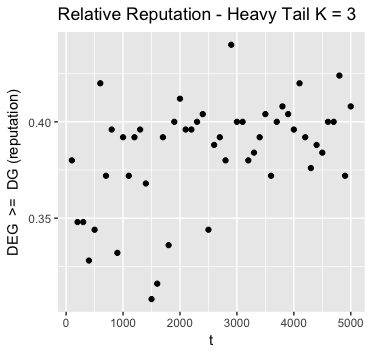
\includegraphics[scale=0.5]{deg_dg_ht_3_prelim}

\section*{Large Warm Start}

We want to see if, for sufficiently large warm start, we indeed see that TS wins. First, let's take a look at the relative reputation plots for Heavy Tail and Uniform. Notice that, for both, $DEG, DG > TS$ in the earlier time horizons and $TS > DEG, DG$ in the later time horizons, with Uniform taking longer for $TS > DEG, DG$ than Heavy Tail. \\

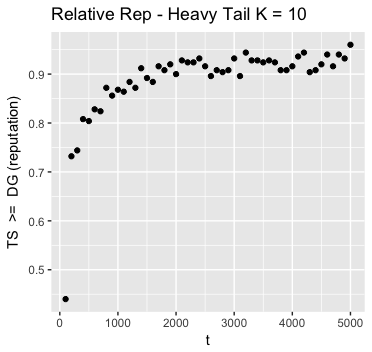
\includegraphics[scale=0.5]{ts_dg_ht_prelim_10} \\
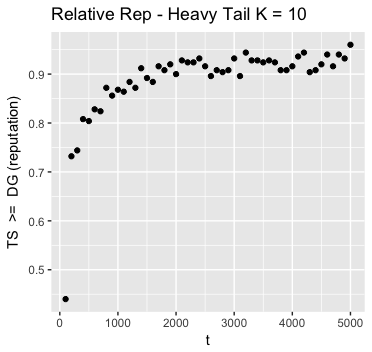
\includegraphics[scale=0.5]{ts_deg_ht_10_prelim} \\
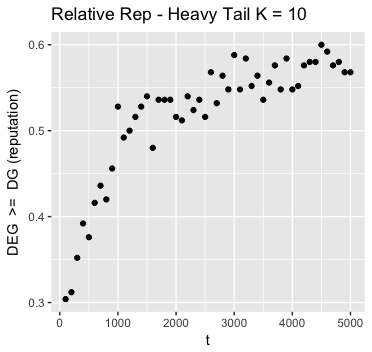
\includegraphics[scale=0.4]{deg_dg_ht_10_prelim} \\
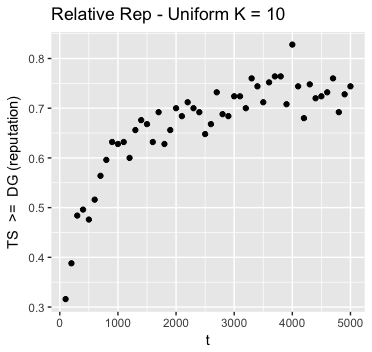
\includegraphics[scale=0.5]{ts_dg_uniform_10_prelim} \\
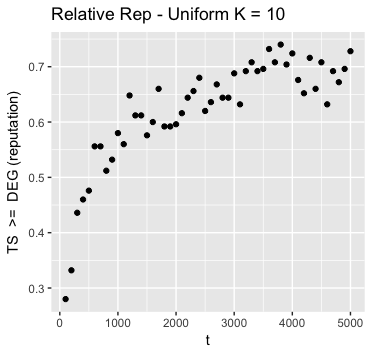
\includegraphics[scale=0.5]{ts_deg_unif_10_prelim} \\
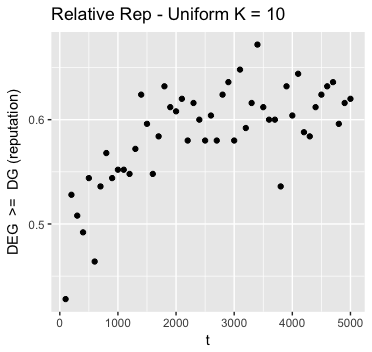
\includegraphics[scale=0.4]{deg_dg_unif_10_prelim} \\

Given this we conjectured that in the competition game, $DEG, DG > TS$ in the early rounds but $TS > DEG, DG$. This largely seems to be the case. See the results below. Additionally, here are two more preliminary plots with smaller time gaps.

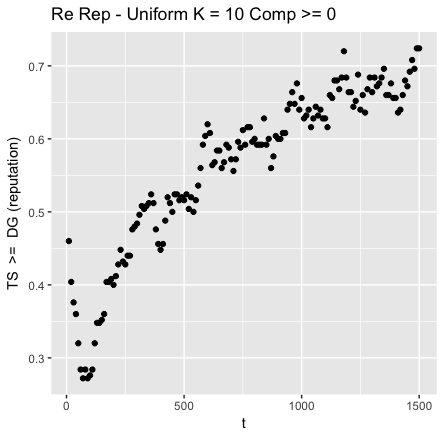
\includegraphics[scale=0.5]{ts_dg_unif_fine} \\
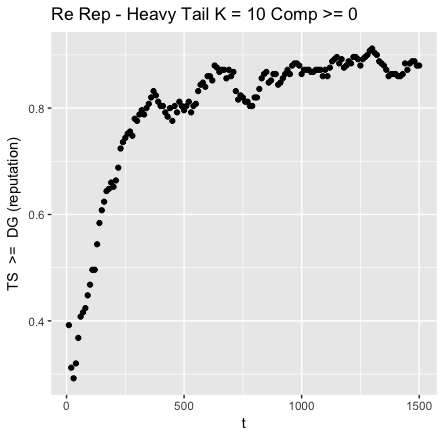
\includegraphics[scale=0.5]{ts_dg_heavy_fine} \\

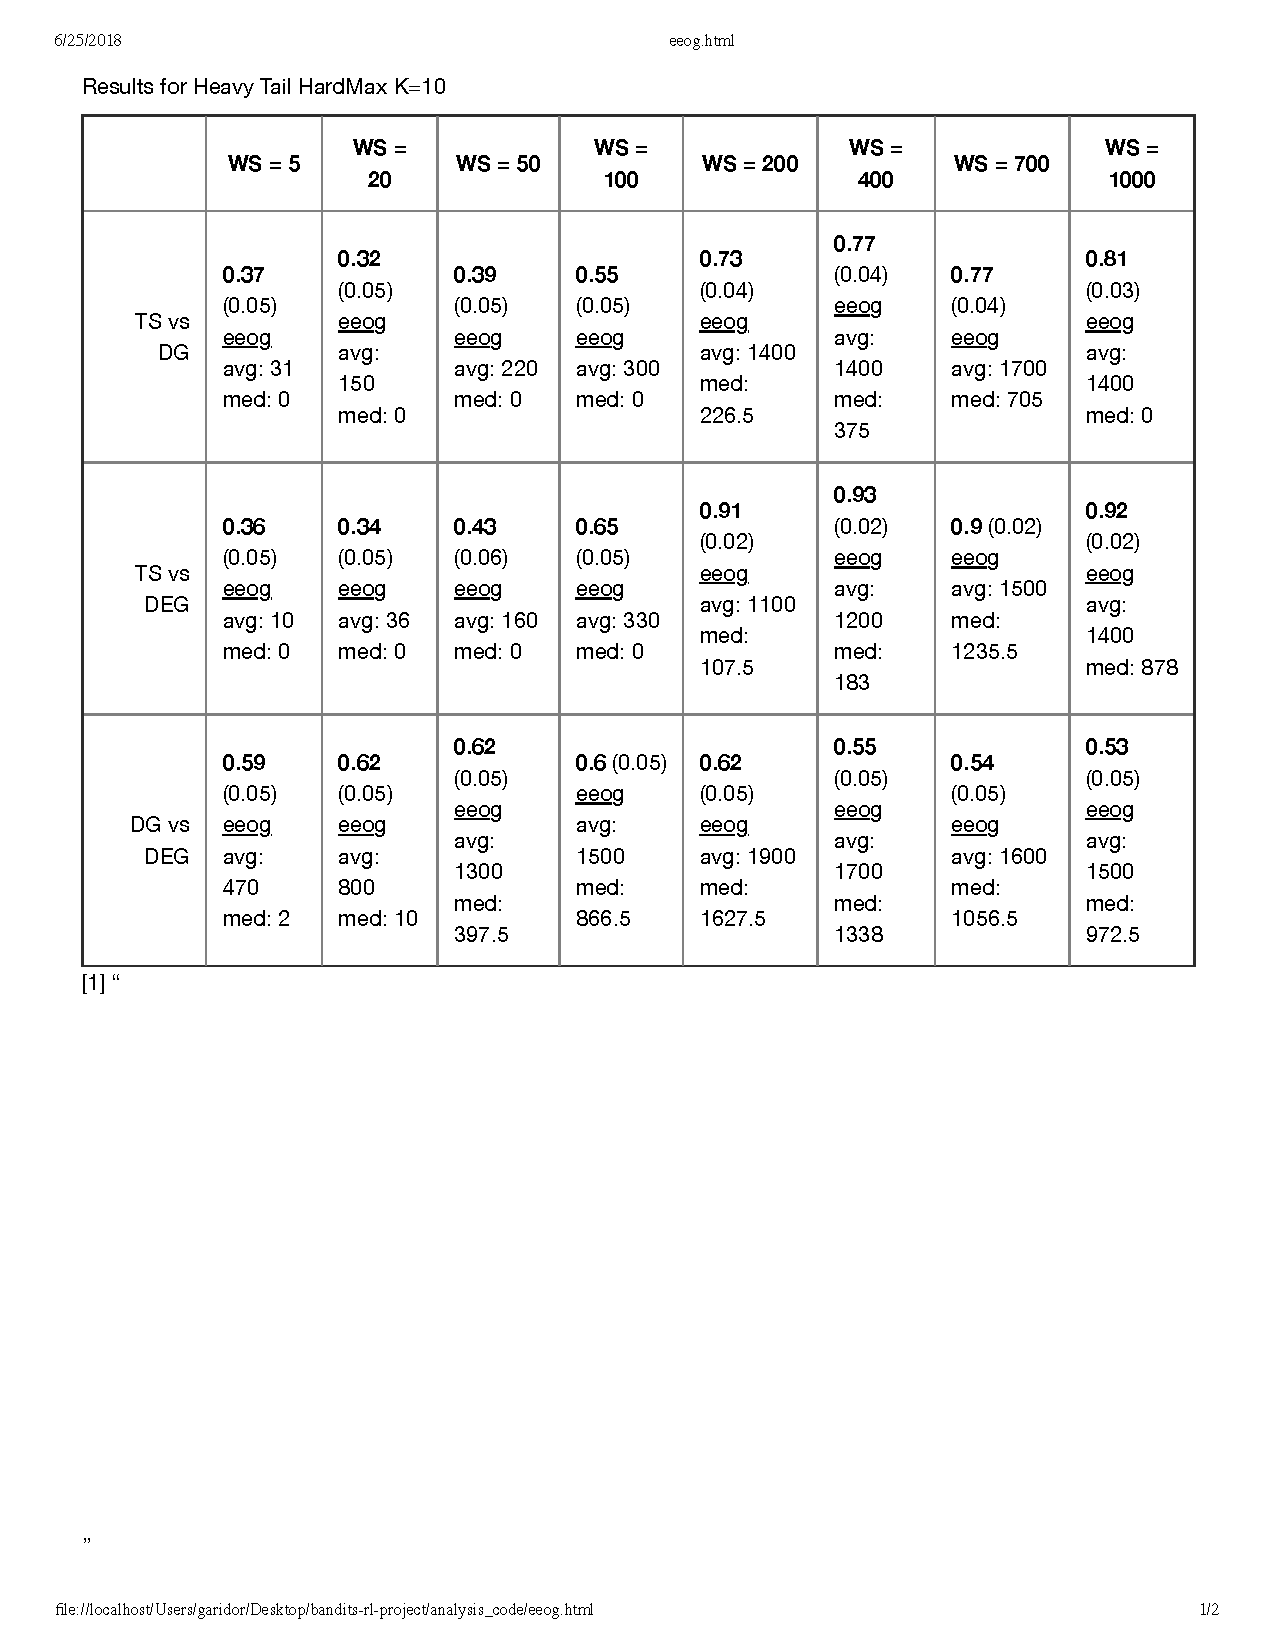
\includepdf[pages={-}]{large_ws}

\section*{Learning Complexity}

Using the same instances that we used for the plots generated in the preliminary plots, we calculate the empirical ``learning complexity" for the $K = 10$ instances according to the hardness metric defined above.

\vspace{0.5cm}
\noindent \underline{Needle In Haystack - 0.5} \\ \textbf{Mean}:  45 \textbf{Median} : 45 \\
\underline{Heavy Tail} \\ \textbf{Mean}:  196.897  \textbf{Median} : 49.08325 \\
\underline{.5/.7 Random Draw} \\ \textbf{Mean}:  23.82 \textbf{Median}: 25  \\
\underline{Uniform} \\ \textbf{Mean}:  171.7698 \textbf{Median} : 79.59571  \\

\vspace{0.5cm}
This is promising given that Heavy Tail and Uniform are the two instances where we see that $DEG, DG > TS$ for HardMax since before we conjectured that on harder learning instances, for small enough warm start observations, TS will do purposeful exploration and get bad reputation and thus lose the competition game. There is probably more we should validate about this metric but need to think about it more.

One puzzling thing about it is, for instance, on the easy instance of 0.5 / 0.7 Random Draw, we see that things are roughly 50 / 50 but we see that $TS > DEG, DG$ on Needle In Haystack - 0.5? One idea is that on 0.5 / 0.7 learning is so easy that there is no value to smarter exploration and that on Needle In Haystack learning is not trivial but is very quick  so that only a few samples are needed and thus the reputational cost is negligible but since $DG$ can't trivially find the best arm there is value to smarter exploration. Not sure though.

\section*{Incumbent Experiment - Varying the number of free observations}

Another implication of the proposed conjectures is that TS ought to be the dominant strategy for the incumbent as long as they are an incumbent for sufficiently long before the entrant enters the market. We fix the agent response model as HardMax. Then, for sufficiently hard learning problems it ought to be the case that if the incumbent only has relatively few periods as the monopolist then TS will not necessarily win. However, with sufficiently long time as the monopolist then TS ought to win.

We verify this in two experiments by first looking where the incumbent gets 50 free observations and then where the incumbent gets 200 free observations. We observe that in the case of 50 free observations, TS does not beat DEG and DG from the ``harder" instances defined by the complexity metric defined above (i.e. Uniform and Heavy Tail), wins in the relatively easier but not trivial learning problem NIH, and algorithm choice makes little difference in the 0.5 / 0.7 Prior.

When we increase the number of free observations to 200 we see that TS is a better algorithm choice for the incumbent (one exception - Uniform against DEG but this is likely due to the fact that we need more free observations, see the preliminary plots).

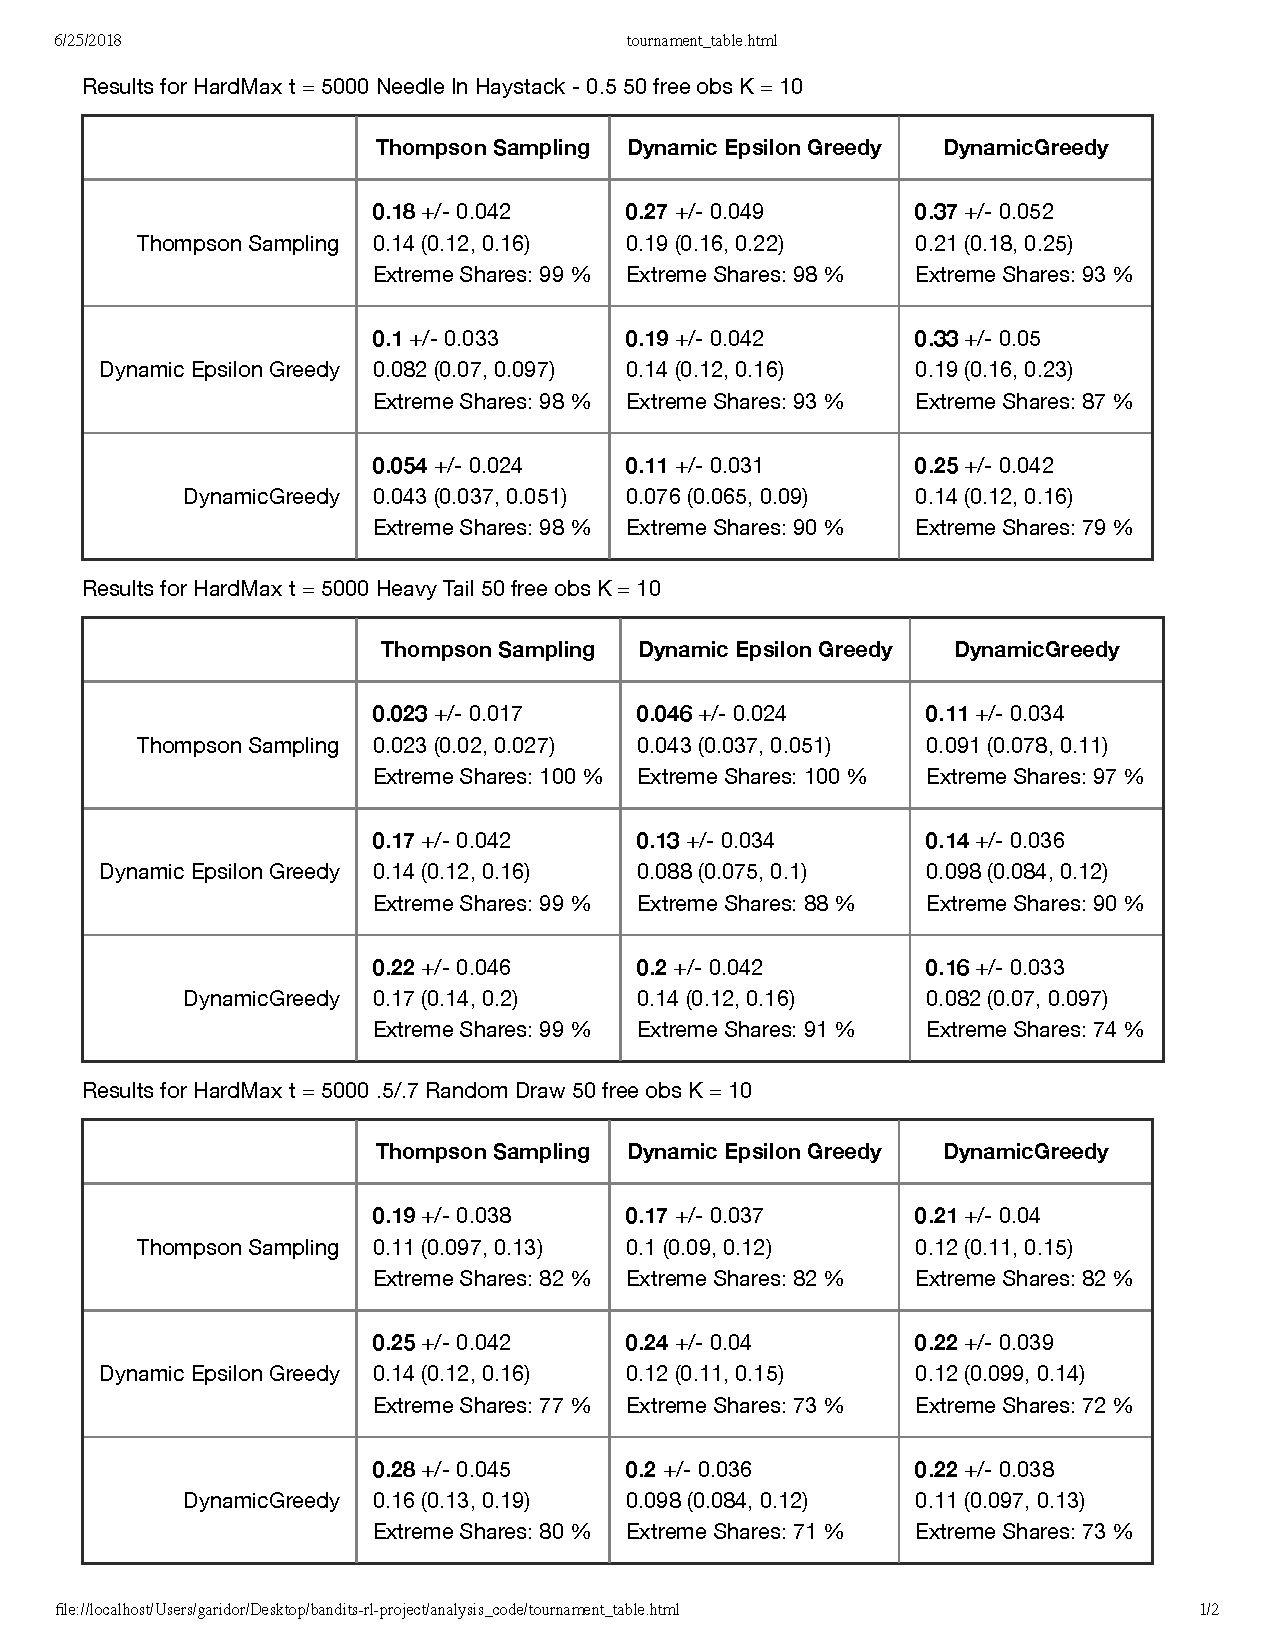
\includepdf[pages={-}]{free_obs_50_10_arms}


\section*{Appendix}

The rest of the relative reputation plots: \\
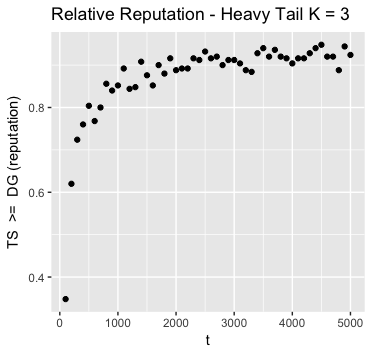
\includegraphics[scale=0.5]{ts_dg_ht_3_prelim} \\
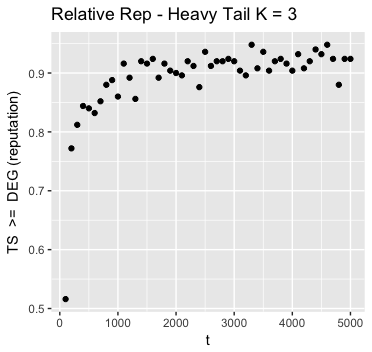
\includegraphics[scale=0.5]{ts_deg_ht_3_prelim} \\
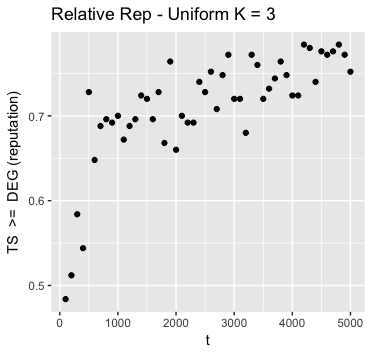
\includegraphics[scale=0.5]{ts_deg_unif_3_prelim} \\
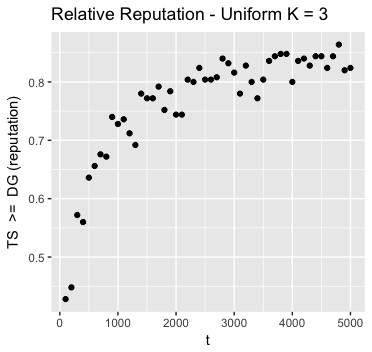
\includegraphics[scale=0.5]{ts_dg_unif_3_prelim} \\
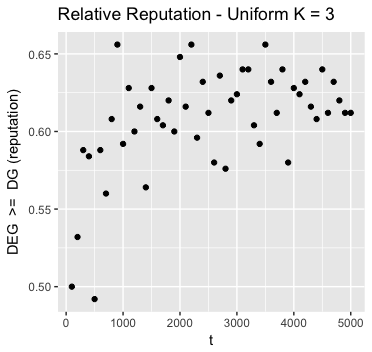
\includegraphics[scale=0.5]{deg_dg_unif_3_prelim} \\

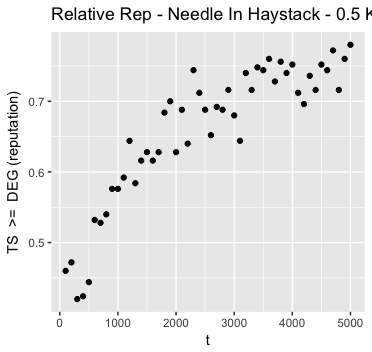
\includegraphics[scale=0.5]{ts_deg_nih_10_prelim} \\
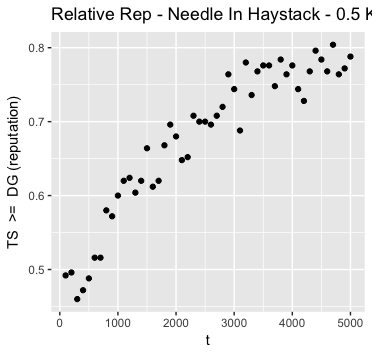
\includegraphics[scale=0.5]{ts_dg_nih_10_prelim} \\
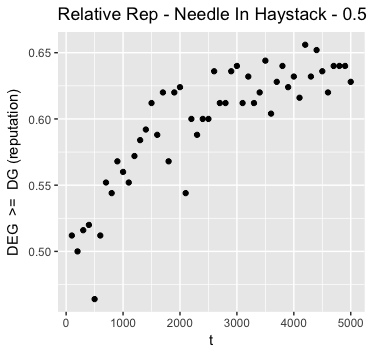
\includegraphics[scale=0.5]{deg_dg_nih_10_prelim} \\
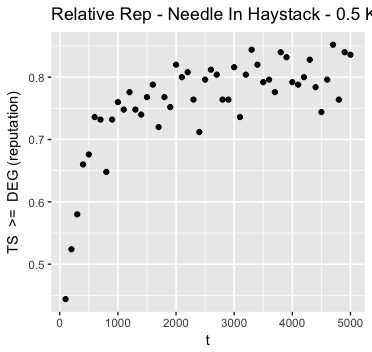
\includegraphics[scale=0.5]{ts_deg_nih_3_prelim} \\
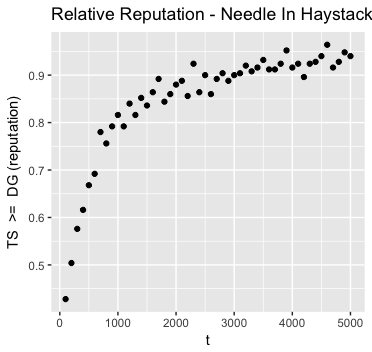
\includegraphics[scale=0.5]{ts_dg_nih_3_prelim} \\
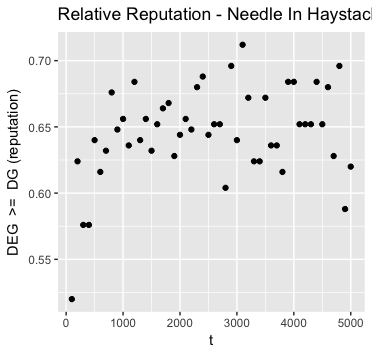
\includegraphics[scale=0.5]{deg_dg_nih_3_prelim} \\

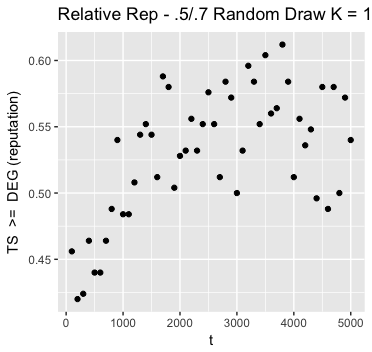
\includegraphics[scale=0.5]{ts_deg_5_7_10_prelim} \\
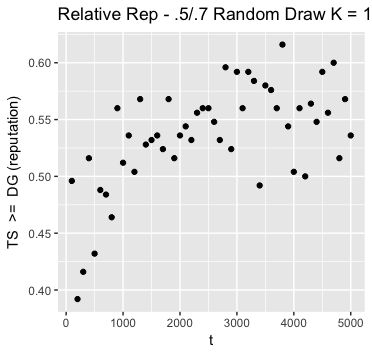
\includegraphics[scale=0.5]{ts_dg_5_7_10_prelim} \\
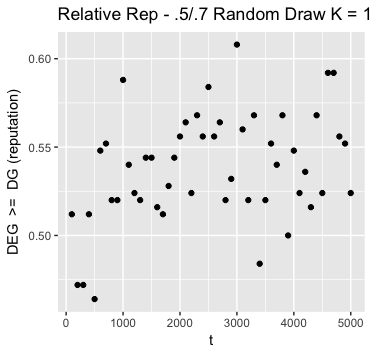
\includegraphics[scale=0.5]{deg_dg_5_7_10_prelim} \\

Finally, here is the warm start experiment redone with reputation erased after the warm start:

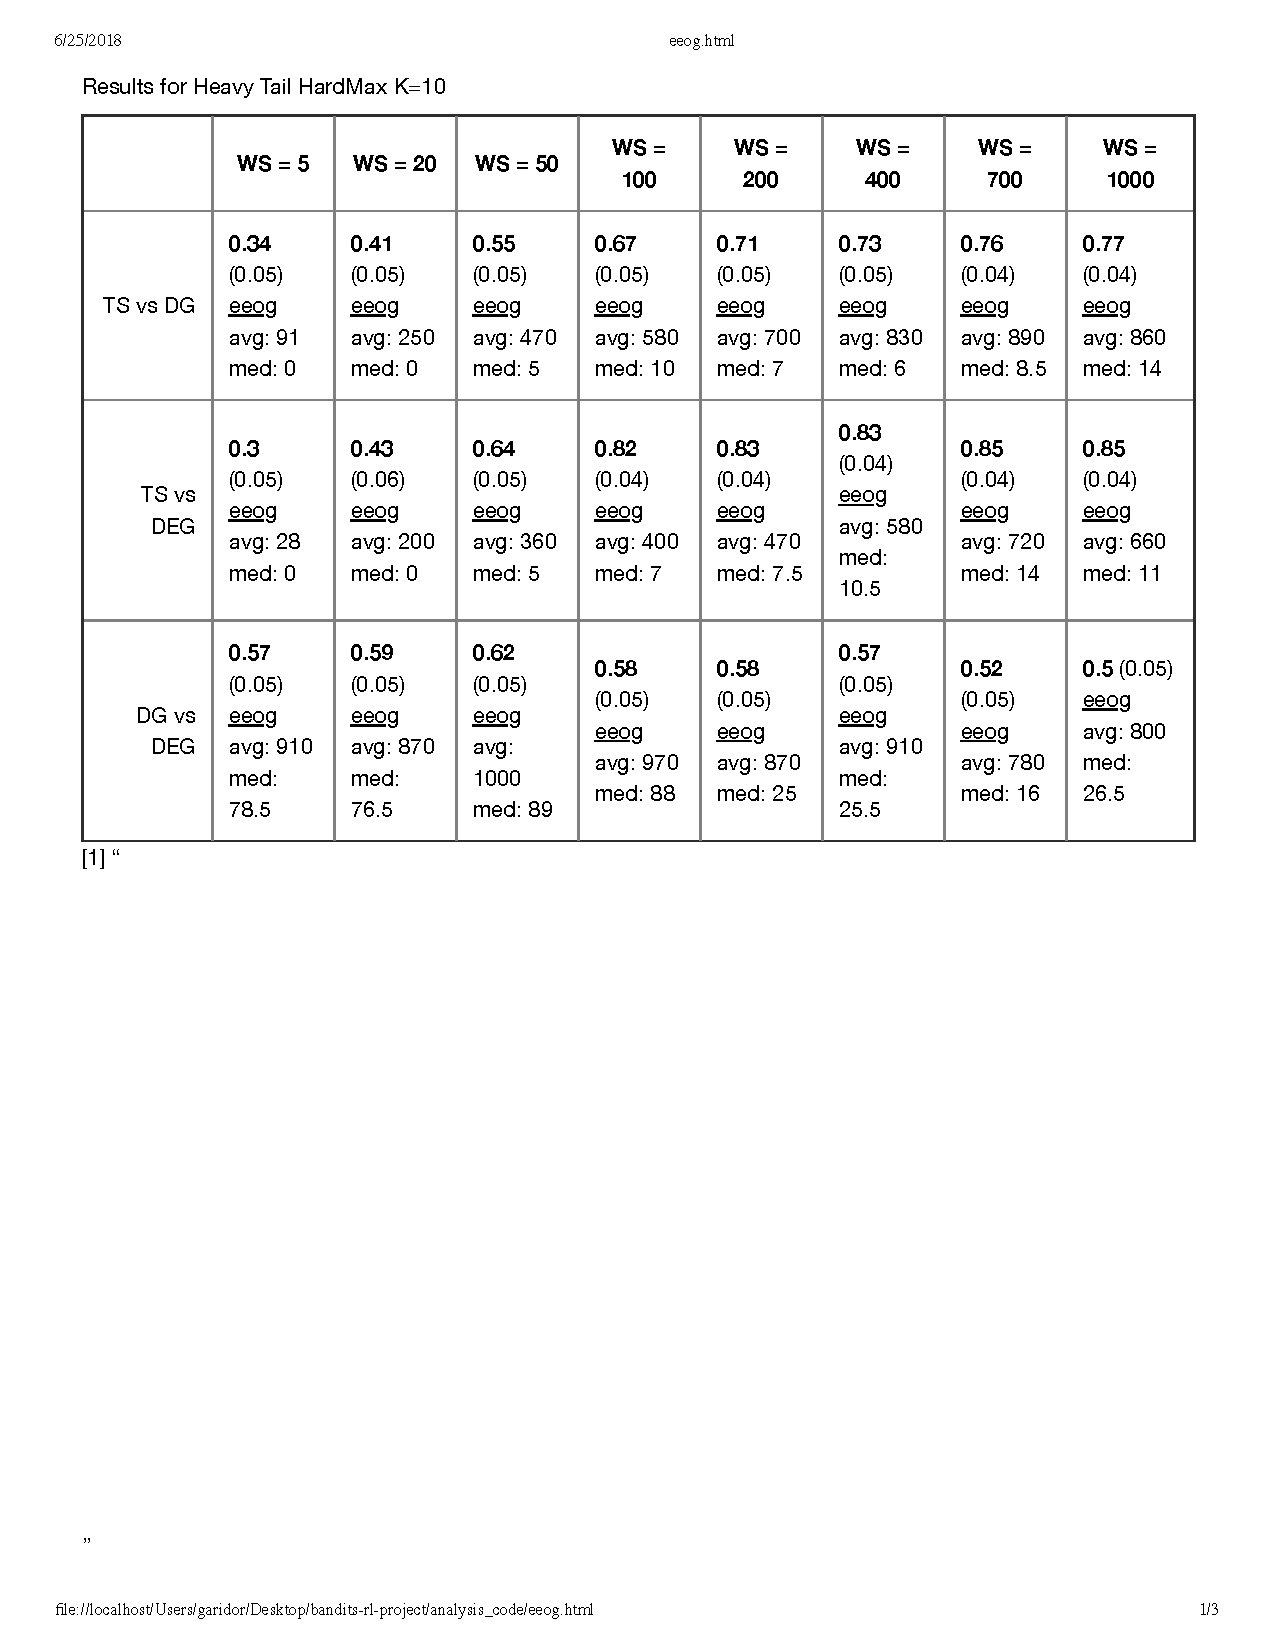
\includepdf[pages={-}]{large_ws_erase_rep}

\end{document}